\section{Propuesta 3}
\label{sec:propuesta_3}

    La propuesta 2 (Sección~\ref{sec:propuesta_2}) acota el tiempo que el servicio permanece caído, pero no evita la caída:
    la request inválida sigue terminando el proceso cada vez que llega (Figura~\ref{fig:comparacion_propuesta_2_sistema_base_chaos_requests_state}).
    Además, ninguna de las propuestas anteriores resuelve los problemas de correctitud de los saldos identificados en el análisis
    del código (Sección~\ref{sec:impacto_en_la_confiabilidad}). La propuesta 3 ataca la causa de estas fallas en lugar de sus efectos.

    Para ello aplicamos las siguientes tácticas:

    \begin{itemize}
        \item \textbf{Validación de entradas (seguridad, prevención de fallas):} la API valida tipos, rangos y monedas soportadas
        antes de procesar cada request, y rechaza con HTTP 400 las que no cumplen. Se reemplaza la validación por presencia
        del sistema base (Código~\ref{lst:request_validation}).
        \item \textbf{Manejo de excepciones (disponibilidad):} los handlers capturan los errores no previstos y responden HTTP 500
        sin terminar el proceso. Además, los rechazos de negocio (por ejemplo, falta de fondos) pasan a informarse como errores
        del cliente (4xx) en lugar de 500.
        \item \textbf{Reserva de saldo (confiabilidad):} el saldo de la cuenta interna se descuenta antes de iniciar las
        transferencias y se devuelve si alguna falla. De esta forma, la verificación y el descuento ocurren sin un \texttt{await}
        intermedio, eliminando la condición de carrera del Código~\ref{lst:race_condition}.
    \end{itemize}

    \todo{Confirmar el alcance final: si se agrega redondeo explícito de importes (Código~\ref{lst:floats}), sumarlo como táctica.}

    Al igual que la propuesta 2, esta propuesta se implementó sobre el sistema base, de modo que los resultados solo reflejan
    el efecto de estas tácticas y sean comparables contra el sistema base.

    Esta propuesta no altera la arquitectura: no agrega componentes ni conectores, por lo que el diagrama Components \&
    Connectors es el mismo que el del sistema base (Figura~\ref{fig:sistema_base_componentes_y_conectores}). Los cambios se
    limitan al código de la API.

    \todo{Agregar los fragmentos de código de la implementación (validación, manejo de errores y reserva de saldo) como bloques \texttt{code} en \texttt{latex/code/}.}

    \subsection{Impacto en los QA}
    \label{sec:propuesta_3_impacto_en_los_qa}

        \subsubsection{Disponibilidad}
        \label{sec:propuesta_3_disponibilidad}

        Es uno de los QA que la propuesta busca mejorar. A diferencia de la propuesta 2, que detecta la falla y se recupera, esta
        propuesta la previene: una request inválida es rechazada antes de acceder a tasas o cuentas inexistentes, y un error no
        previsto queda contenido en la request que lo produjo en lugar de terminar el proceso.

        \todo{Completar con la evidencia del escenario de caos (Sección~\ref{sec:propuesta_3_pruebas_de_chaos}).}

        La táctica solo cubre las fallas originadas por el procesamiento de una request. Una terminación del proceso por otras
        causas (falta de memoria, error del runtime o del host) sigue dejando el servicio caído, por lo que es complementaria
        con la propuesta 2.

        \subsubsection{Confiabilidad}
        \label{sec:propuesta_3_confiabilidad}

        Es el otro QA que la propuesta busca mejorar. La reserva de saldo garantiza que dos operaciones concurrentes no puedan
        aprobarse con el mismo saldo, por lo que la cuenta interna no puede quedar en negativo.

        \todo{Completar con la evidencia del escenario de concurrencia (Sección~\ref{sec:propuesta_3_pruebas_de_concurrencia}).}

        Como contrapartida, mientras una operación está en curso el saldo reservado no está disponible para otras, por lo que
        una operación que luego falla puede provocar el rechazo de otra que sí tenía fondos. Consideramos preferible rechazar
        una operación válida antes que aprobar una que deje un saldo negativo.

        La propuesta no resuelve la durabilidad diferida ni la escritura no atómica del estado (Código~\ref{lst:save}).

        \subsubsection{Seguridad}
        \label{sec:propuesta_3_seguridad}

        La validación impide que un consumidor que invoque directamente la API altere los saldos con importes negativos o
        provoque una denegación de servicio con una request malformada, que en el sistema base alcanzaba para tirar el
        servicio (Sección~\ref{sec:sistema_base_pruebas_de_chaos}).

        \todo{Agregar evidencia de ejecución: request con importe negativo y con moneda inexistente, base vs propuesta 3.}

        \subsubsection{Performance}
        \label{sec:propuesta_3_performance}

        La validación agrega comprobaciones en memoria de costo constante por request, que consideramos despreciables frente a
        los 400 a 800ms de las transferencias. La reserva de saldo no agrega esperas, ya que no utiliza un lock. No se espera que
        la propuesta mejore la degradación producida por el log, que se mantiene igual que en el sistema base.

        \todo{Confirmar con las pruebas de estrés y resistencia (Secciones~\ref{sec:propuesta_3_pruebas_de_stress} y~\ref{sec:propuesta_3_pruebas_de_soak}).}

        \subsubsection{Modificabilidad}
        \label{sec:propuesta_3_modificabilidad}

        \todo{Discutir: las reglas de validación quedan acopladas a las monedas y cuentas existentes; agregar una moneda requiere actualizar la validación. Mencionar si la validación queda centralizada en un módulo.}

        \subsubsection{Testeabilidad}
        \label{sec:propuesta_3_testeabilidad}

        \todo{Discutir: la validación separada de la lógica de cambio puede probarse de forma aislada; los códigos de respuesta 4xx/5xx permiten distinguir errores del cliente de fallas del servidor.}

        \subsubsection{Simplicidad}
        \label{sec:propuesta_3_simplicidad}

        Es la propuesta de menor complejidad: no agrega componentes, conectores ni dependencias de despliegue, y los cambios se
        concentran en la API. El costo es un aumento del código de la API y de la cantidad de casos que deben contemplarse al
        modificarla.

    \subsection{Pruebas de carga}
    \label{sec:propuesta_3_pruebas_de_baseline}

    Las pruebas de carga comparten la misma configuración con el sistema base de tal forma que los resultados sean comparables, ver Sección~\ref{sec:sistema_base_pruebas_de_baseline}.

    \todo{Describir brevemente los resultados o eliminar la subsección y dejar solo la referencia al apéndice.}

    Se pueden encontrar los resultados completos en el Apéndice (Sección~\ref{sec:resultados_completos_propuesta_3_baseline}).

    \subsection{Pruebas de estrés}
    \label{sec:propuesta_3_pruebas_de_stress}

    Las pruebas de estrés comparten la misma configuración con el sistema base de tal forma que los resultados sean comparables, ver Sección~\ref{sec:sistema_base_pruebas_de_stress}.
    En este escenario no hay requests inválidas, por lo que esperamos que la propuesta no presente diferencias frente al sistema base.

    Se pueden encontrar los resultados completos en el Apéndice (Sección~\ref{sec:resultados_completos_propuesta_3_stress}).

        \subsubsection{Latencia}
        \label{sec:propuesta_3_pruebas_de_stress_metricas_latencia}

            \begin{figure}[H]
                \centering
                % TODO: reemplazar por figures/propuesta_3/stress/endpoint_response_time
                
\includegraphics[width=0.5\columnwidth]{figures/placeholder}%
                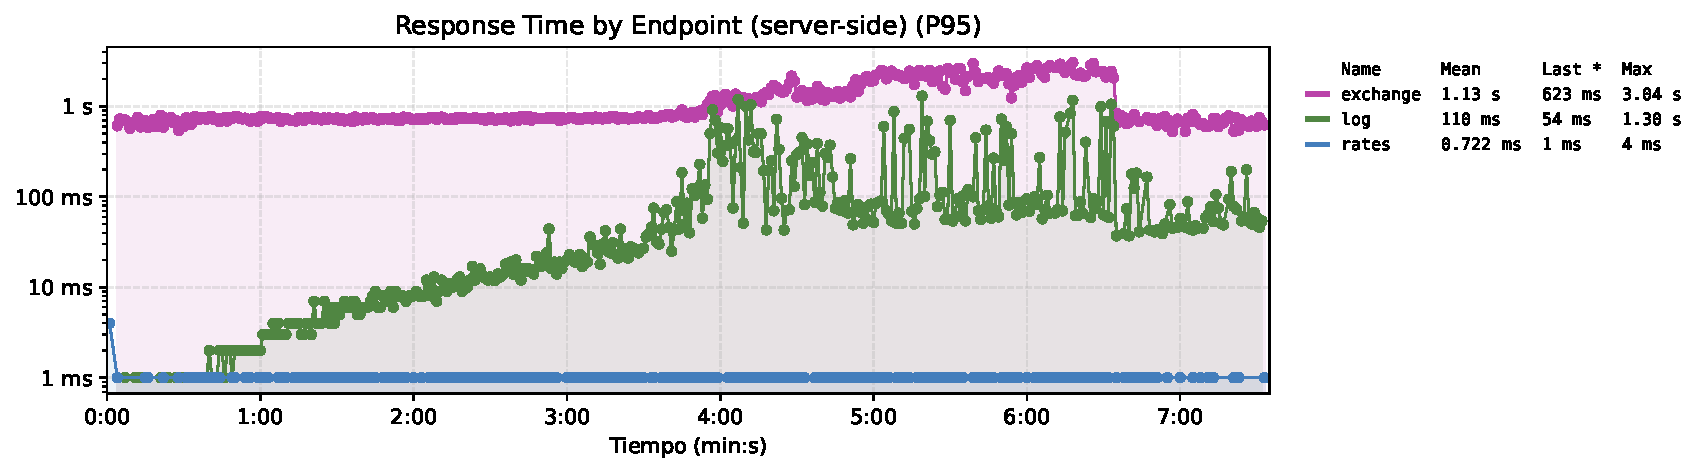
\includegraphics[width=0.5\columnwidth]{figures/sistema_base/stress/endpoint_response_time}
                \caption{
                    Comparativa de los resultados de latencia por endpoint entre la propuesta 3 (izquierda) y el sistema base (derecha) frente a un escenario de estrés.
                    \todo{Completar.}
                }
                \label{fig:comparacion_propuesta_3_sistema_base_stress_endpoint_response_time}
            \end{figure}

        \subsubsection{Uso de recursos}
        \label{sec:propuesta_3_pruebas_de_stress_metricas_recursos}

            \begin{figure}[H]
                \centering
                % TODO: reemplazar por figures/propuesta_3/stress/resources
                
\includegraphics[width=0.5\columnwidth]{figures/placeholder}%
                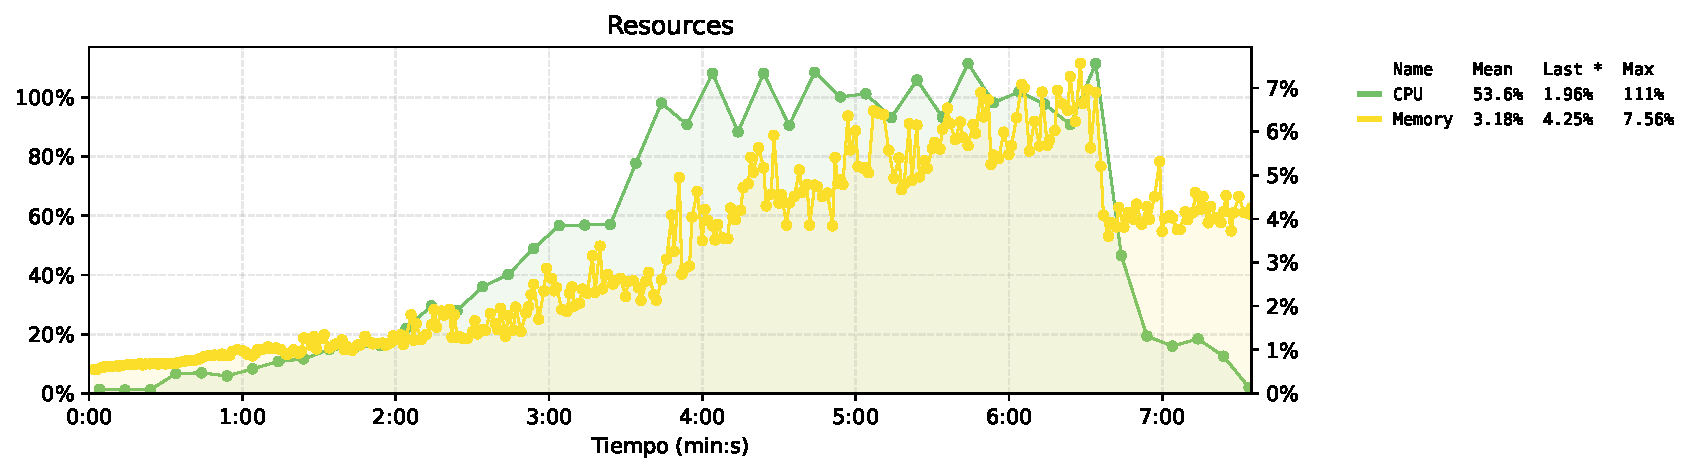
\includegraphics[width=0.5\columnwidth]{figures/sistema_base/stress/resources}
                \caption{
                    Comparativa de los resultados del uso de recursos entre la propuesta 3 (izquierda) y el sistema base (derecha) frente a un escenario de estrés.
                    \todo{Completar.}
                }
                \label{fig:comparacion_propuesta_3_sistema_base_stress_resources}
            \end{figure}

    \subsection{Pruebas de resistencia}
    \label{sec:propuesta_3_pruebas_de_soak}

    Las pruebas de resistencia comparten la misma configuración con el sistema base de tal forma que los resultados sean comparables, ver Sección~\ref{sec:sistema_base_pruebas_de_soak}.
    Al igual que en el escenario de estrés, no esperamos diferencias frente al sistema base.

    Se pueden encontrar los resultados completos en el Apéndice (Sección~\ref{sec:resultados_completos_propuesta_3_soak}).

        \subsubsection{Disponibilidad}
        \label{sec:propuesta_3_pruebas_de_soak_metricas_disponibilidad}

            \begin{figure}[H]
                \centering
                % TODO: reemplazar por figures/propuesta_3/soak/requests_state
                
\includegraphics[width=0.5\columnwidth]{figures/placeholder}%
                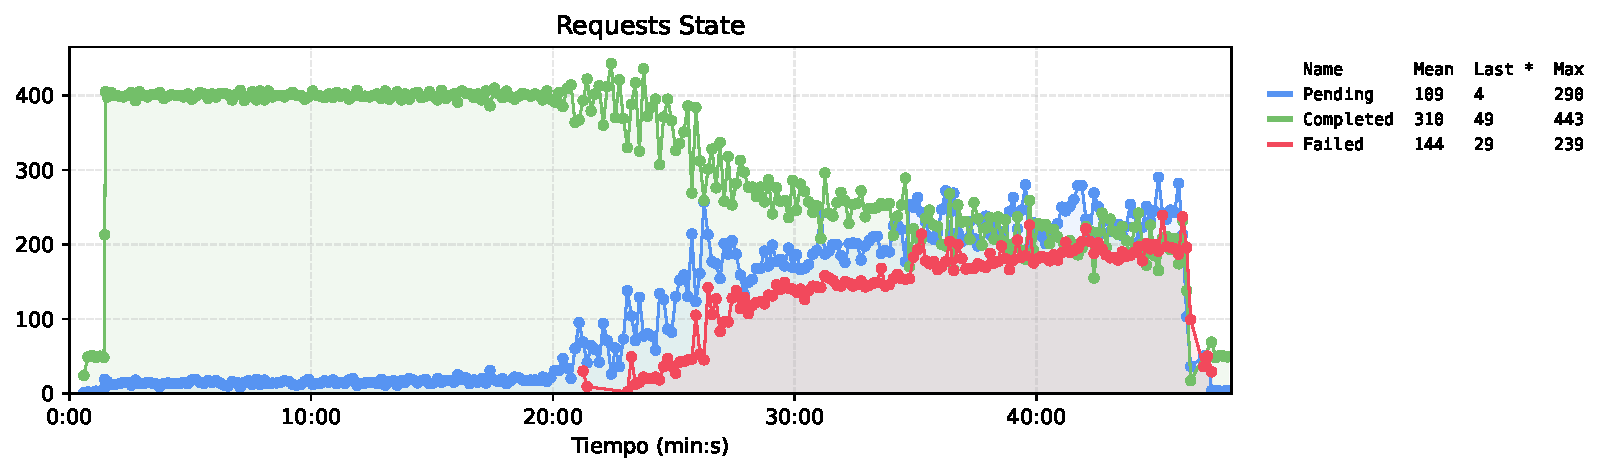
\includegraphics[width=0.5\columnwidth]{figures/sistema_base/soak/requests_state}
                \caption{
                    Comparativa de la disponibilidad ofrecida por la propuesta 3 (izquierda) y el sistema base (derecha) frente a un escenario de resistencia.
                    \todo{Completar.}
                }
                \label{fig:comparacion_propuesta_3_sistema_base_soak_requests_state}
            \end{figure}

        \subsubsection{Latencia}
        \label{sec:propuesta_3_pruebas_de_soak_metricas_latencia}

            \begin{figure}[H]
                \centering
                % TODO: reemplazar por figures/propuesta_3/soak/endpoint_response_time
                
\includegraphics[width=0.5\columnwidth]{figures/placeholder}%
                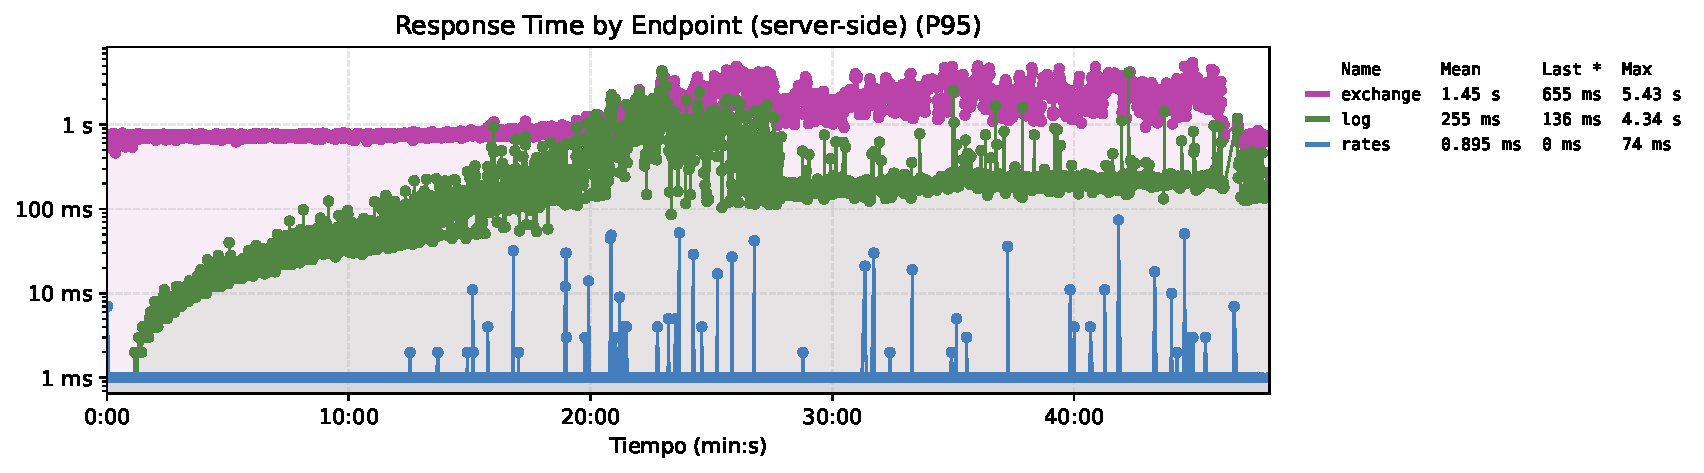
\includegraphics[width=0.5\columnwidth]{figures/sistema_base/soak/endpoint_response_time}
                \caption{
                    Comparativa de los resultados de latencia por endpoint entre la propuesta 3 (izquierda) y el sistema base (derecha) frente a un escenario de resistencia.
                    \todo{Completar.}
                }
                \label{fig:comparacion_propuesta_3_sistema_base_soak_endpoint_response_time}
            \end{figure}

    \subsection{Pruebas de caos}
    \label{sec:propuesta_3_pruebas_de_chaos}

    Las pruebas de caos comparten la misma configuración con el sistema base de tal forma que los resultados sean comparables, ver Sección~\ref{sec:sistema_base_pruebas_de_chaos}.
    La request inválida utiliza una moneda inexistente (\texttt{XXX}). Este es el escenario en el que esperamos ver el efecto de la
    validación y del manejo de excepciones: el sistema no debería caer y la request inválida debería rechazarse con HTTP 400.

    Se pueden encontrar los resultados completos en el Apéndice (Sección~\ref{sec:resultados_completos_propuesta_3_chaos}).

        \subsubsection{Disponibilidad}
        \label{sec:propuesta_3_pruebas_de_chaos_metricas_disponibilidad}

            \begin{figure}[H]
                \centering
                % TODO: reemplazar por figures/propuesta_3/chaos/requests_state
                
\includegraphics[width=0.5\columnwidth]{figures/placeholder}%
                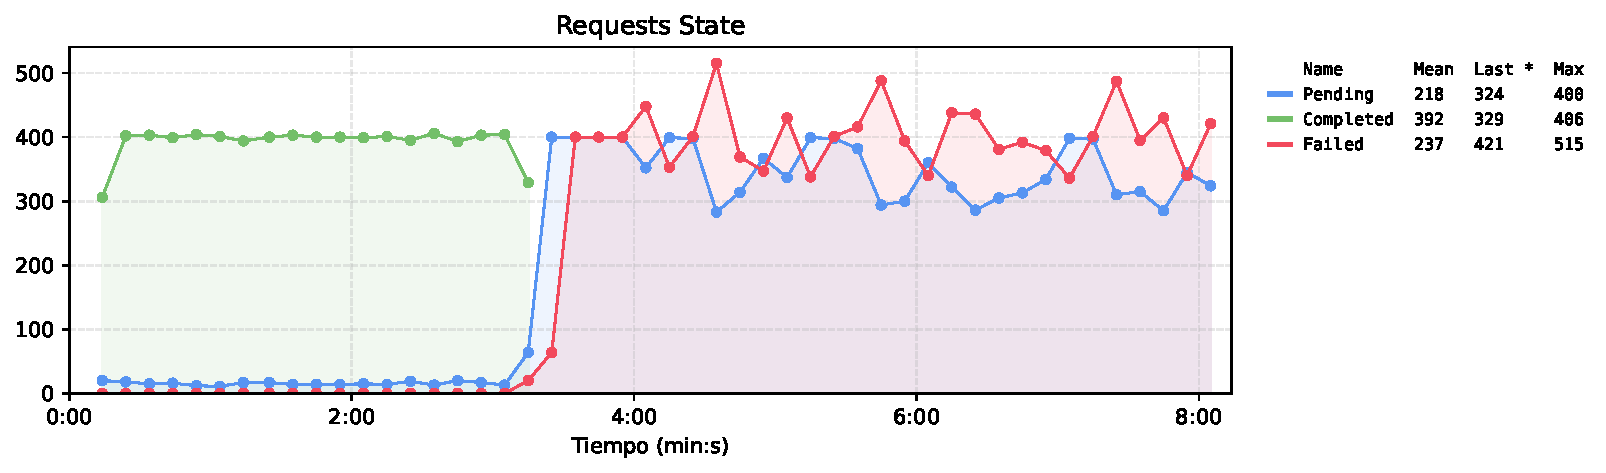
\includegraphics[width=0.5\columnwidth]{figures/sistema_base/chaos/requests_state}
                \caption{
                    Comparativa de la disponibilidad ofrecida por la propuesta 3 (izquierda) y el sistema base (derecha) frente a un escenario de caos.
                    \todo{Completar. Comparar también con la propuesta 2 (Figura~\ref{fig:comparacion_propuesta_2_sistema_base_chaos_requests_state}): P2 se recupera de cada caída, P3 no cae.}
                }
                \label{fig:comparacion_propuesta_3_sistema_base_chaos_requests_state}
            \end{figure}

        \subsubsection{Latencia}
        \label{sec:propuesta_3_pruebas_de_chaos_metricas_latencia}

            \begin{figure}[H]
                \centering
                % TODO: reemplazar por figures/propuesta_3/chaos/response_time
                
\includegraphics[width=0.5\columnwidth]{figures/placeholder}%
                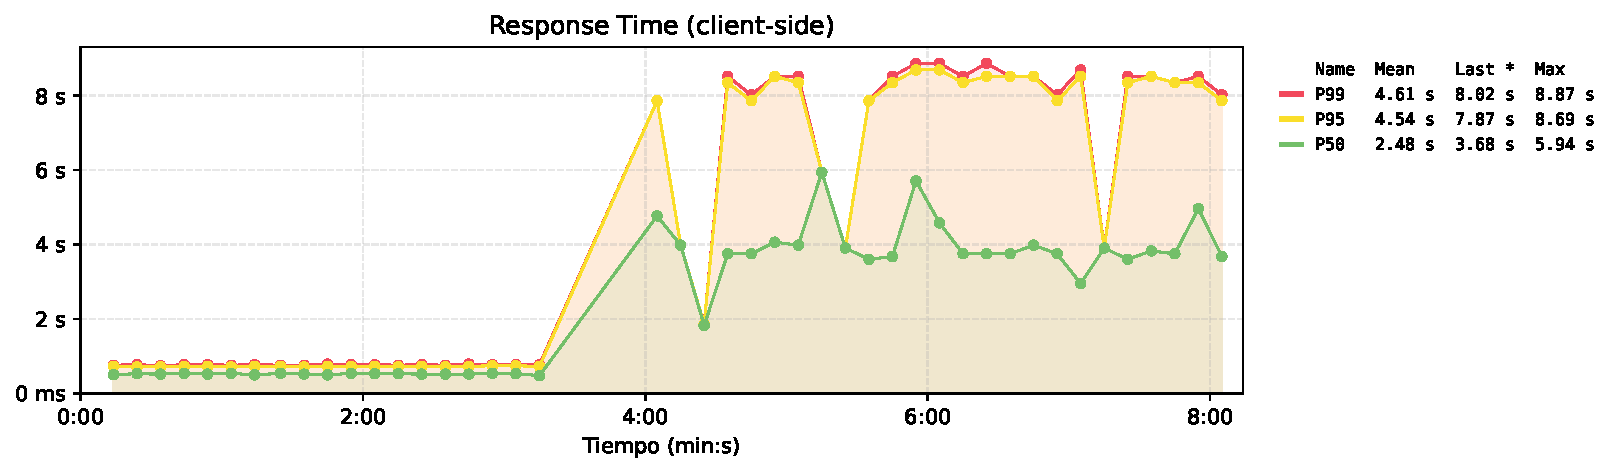
\includegraphics[width=0.5\columnwidth]{figures/sistema_base/chaos/response_time}
                \caption{
                    Comparativa de los resultados de latencia entre la propuesta 3 (izquierda) y el sistema base (derecha) frente a un escenario de caos.
                    \todo{Completar. Esperado: sin picos, a diferencia de la propuesta 2.}
                }
                \label{fig:comparacion_propuesta_3_sistema_base_chaos_response_time}
            \end{figure}

        \subsubsection{Volumen operado por moneda}
        \label{sec:propuesta_3_pruebas_de_chaos_metricas_volumen_operado_por_moneda}

            \begin{figure}[H]
                \centering
                % TODO: reemplazar por figures/propuesta_3/chaos/currency
                
\includegraphics[width=0.5\columnwidth]{figures/placeholder}%
                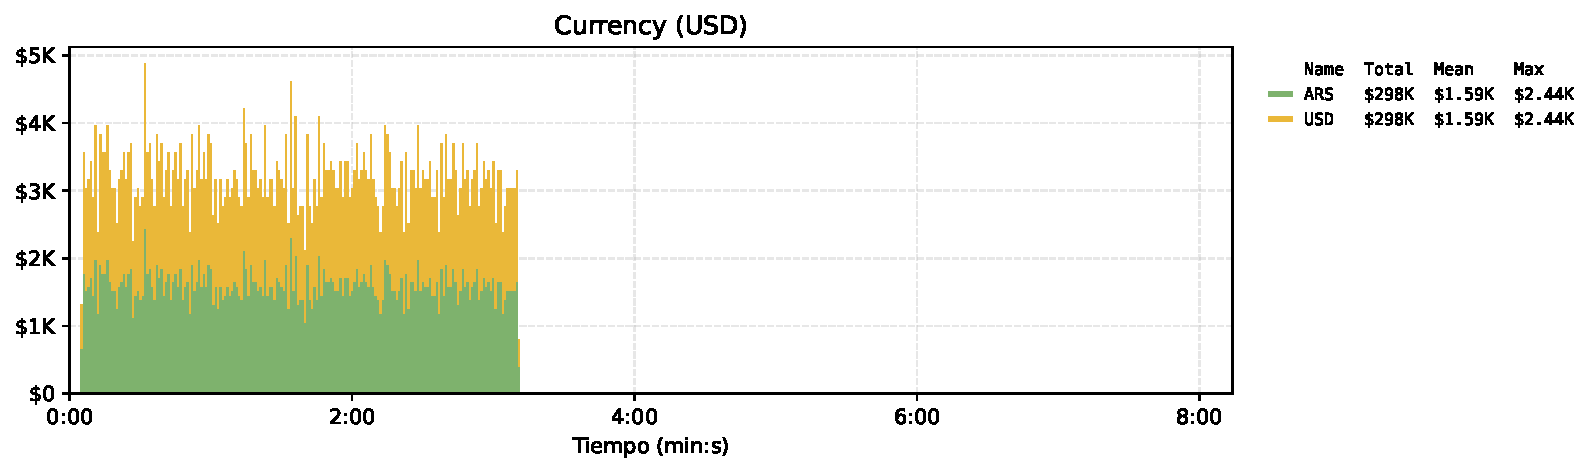
\includegraphics[width=0.5\columnwidth]{figures/sistema_base/chaos/currency}
                \caption{
                    Comparativa de los resultados de volumen operado en cada moneda entre la propuesta 3 (izquierda) y el sistema base (derecha) frente a un escenario de caos.
                    \todo{Completar con el total y el porcentaje frente al base (\$298K) y a la propuesta 2 (\$750K).}
                }
                \label{fig:comparacion_propuesta_3_sistema_base_chaos_currency}
            \end{figure}

    \subsection{Pruebas de concurrencia}
    \label{sec:propuesta_3_pruebas_de_concurrencia}

    \todo{Describir el escenario (\texttt{perf/race.yaml}): saldo inicial de la cuenta interna, cantidad y monto de los \texttt{/exchange} concurrentes, y por qué el saldo total solicitado supera al disponible.}

    Este escenario se ejecuta tanto sobre el sistema base como sobre la propuesta 3, ya que tiene como objetivo evidenciar la
    condición de carrera identificada en el Código~\ref{lst:race_condition}.

        \subsubsection{Saldo de la cuenta interna}
        \label{sec:propuesta_3_pruebas_de_concurrencia_saldo}

        \todo{Mostrar \texttt{GET /accounts} antes y después en ambos sistemas. Esperado: saldo negativo en el base, nunca negativo en la propuesta 3.}

        \subsubsection{Estado de las requests}
        \label{sec:propuesta_3_pruebas_de_concurrencia_requests}

            \begin{figure}[H]
                \centering
                % TODO: reemplazar por figures/propuesta_3/race/requests_state y figures/sistema_base/race/requests_state
                
\includegraphics[width=0.5\columnwidth]{figures/placeholder}%
                
\includegraphics[width=0.5\columnwidth]{figures/placeholder}
                \caption{
                    Comparativa del estado de las requests entre la propuesta 3 (izquierda) y el sistema base (derecha) frente al escenario de concurrencia.
                    \todo{Completar. Esperado: en el base se aprueban más operaciones que las que cubre el saldo; en la propuesta 3 las excedentes se rechazan.}
                }
                \label{fig:comparacion_propuesta_3_sistema_base_race_requests_state}
            \end{figure}

    \subsection{Resultados y conclusiones}
    \label{sec:propuesta_3_resultados_y_conclusiones}

    \todo{Completar con los resultados. Ideas: P3 previene las caídas que P2 recupera y elimina la carrera sobre los saldos, sin costo de performance ni componentes nuevos; no resuelve la degradación del log (P1) ni las caídas por otras causas (P2), por lo que las tres propuestas son complementarias.}
